\documentclass[a4paper,12pt,indent]{article}
\usepackage{ctex}
%\usepackage[toc]{multitoc}%目录,图标两栏
\usepackage{tikz}
\usepackage{xcolor}
\usepackage{tasks}
\usepackage{graphicx}
\usepackage{fontspec}
\usepackage{tcolorbox}
\usepackage{fontawesome}
\usepackage{xtemplate}
\definecolor{Tasks}{RGB}{165,10,17}
\definecolor{Black}{RGB}{153,63,38}
\definecolor{Keycolor}{RGB}{37,138,210}
\usepackage[
left=1.0in,
right=1.0in,
top=1.2in,
bottom=1.2in
]{geometry}
\usepackage{expl3}
\setmainfont{Fandolsong-Regular.otf}
\usepackage{notesetup_document}

\RequirePackage{listings}
\renewcommand{\ttdefault}{cmtt}
\lstdefinestyle{mystyle}
{
basicstyle       =\ttfamily
\lst@ifdisplaystyle\small\fi
}

\lstset{
 basicstyle      =\ttfamily,
 style           =mystyle,
 breaklines      =true
 }

\definecolor{blackg}{RGB}{251,246,225}
\definecolor{frenchplum}{RGB}{190,20,83}
\lstset{
  language       =[LaTeX]TeX,
  texcsstyle     =*\color{red},
  numbers        =left, 
  numberstyle    =\color{Tasks}\tiny, 
  stepnumber     =1, 
  numbersep      =3pt,
  breaklines     =true,
  keywordstyle   =\color{Tasks},
  commentstyle   =\color{gray},
  emph           ={},
  emphstyle      ={\color{orange!60!red}},
  morekeywords   ={*},
  frame          =single,
  tabsize        =2,
  rulecolor      =\color{gray},
  framerule      =0pt,
  columns        =flexible,
  backgroundcolor=\color{white}
}
\usepackage{listings}

\begin{document}
\renewcommand{\contentsname}{目\quad 录} %%%在{document}里面加入该命令,将"contents"变成“目  录”
\renewcommand{\figurename}{图} %%%在{document}里面加入该命令,将"Figure"变成“图”
\renewcommand{\refname}{参考文献} %%%在{document}里面加入该命令,将"Reference"变成“参考文献”
\setlength{\parindent}{2em} %%%在{document}里面加入该命令,然后在需要缩进的段落前加入\indent
\title{\tikz\node[scale=1.2]{\color{gray}\Huge\bfseries
\textcolor{black}{\textcolor{Tasks}{TASKS\ }}\textcolor{cyan}{宏包}\textcolor{orange}{\emph{学习}}\textcolor{cyan}{手册}
};
%\tikz\node[scale=1]  {\Huge\bfseries \textcolor{black}{\textcolor{blue}{Basics}}};
}

\vspace{3cm}

\author{\href{http://www.latexstudio.net}{\textcolor{yellow!30!red}{原著:Yongxue\ \ \ \ 2020年12月20日}}}
\date{\textcolor{black} {\textcolor{blue}{翻译:\ \ 黄旭华\ \ \ \ \ \ 2022年04月01日}}}

%\author{\href{http://www.latexstudio.net}{\textcolor{yellow!30!red}{翻译:黄旭华}}}
%\date{\textcolor{black}{\textcolor{blue}{\bfseries 2022年03月31日}}}


\maketitle

\thispagestyle{empty}

\vspace{1cm}

\tableofcontents

%\begin{multicols}{2}
%  \tableofcontents
%\end{multicols}

\vspace{7cm}

%\hfill \textcolor{black}{\textcolor{blue}{\rule{0.15\textwidth}{1pt}}} \textcolor{black}{\textcolor{Tasks}{To be continued}} \textcolor{black}{\textcolor{Tasks}{(}}\textcolor{black}{\textcolor{blue}{\emph{Basics<English Version}>}}\textcolor{black}{\textcolor{Tasks}{)}}
\clearpage

\section{动机}
%\subsection*{动机 \& 历史}

最初的 \textcolor{Tasks}{TASKS} 是 \textcolor{Tasks}{ExSheets} 宏包的一部分[Nie19]。然而,用户告诉我,可将其作为一个独立的宏包,而不必仅仅为了使用 \textcolor{Tasks}{TASKS} 环境而加载整个 \textcolor{Tasks}{ExSheets} 宏包。这确实有道理。因此我将该环境被提取到一个tasks宏包中。那时,\textcolor{Tasks}{TASKS} 就作为一个独立的宏包分发,也作为 \textcolor{Tasks}{ExSheets} 捆绑包(bundle)的一部分。完全独立的宏包最初的版本是v0.10。从此,该独立宏包与 \textcolor{Tasks}{ExSheets} 的关系成为历史。

使用 tasks 环境的原因是德国数学教科书(尤其是初中教科书)中有一项不成文的规定,即以横向计算而非纵向计算的栏来组织练习。这就是使用 tasks 的主要目的。如果不需要此功能,最好使用传统的 \LaTeX{} 列表和 enumitem 宏包进行定制。

\subsection*{更改}

\begin{itemize}

 \item 不推荐使用 counter-format 选项。现在,标签的设置方式与 enumitem 中的设置方式非常相似。这也使得列表模板的 enumerate 选项变得多余,并相应地被删除。

\item 已重命名 \verb|\|\textcolor{Tasks}{NewTasks} 命令和 \verb|\|\textcolor{Tasks}{RenewTasks} 命令。

\item 已删除多项选择列表(multiple choice lists)。

\item 自定义的定义(custom defnitions)可以放在tasks.cfg文件中,可自动加载该文件(如果可用)。

\end{itemize}

\section{许可证和需要}

根据 \LaTeX{} 项目公共许可证(lppl)1.3c版或更高版本(http://www.latex-project.org/ lppl.txt)的条款,允许复制、分发和/或修改本软件。该软件的状态为“已维护(maintained)”。

\textcolor{Tasks}{TASKS} 需要 l3kernel [L3P] 捆绑包、xparse1和 xtemplate。

\section{如何工作}

\subsection{背景}

\textcolor{Tasks}{TASKS}环境和 enumerate 列表有点相似但不相同,不同之处如下:
\begin{enumerate}
    \item 分页(pagebreak)在一个条目(item)中不可用,但在两个条目(item)间可用。

    \item 计数(enumeration)默认是 a),b),c)

    \item 每次出现条目分隔符(item separator)时,tasks环境的主体都会被拆分。因此,默认的分隔符不是 \verb|\|\textcolor{Tasks}{item},而是\verb|\|\textcolor{Tasks}{task},因此它仅限于该环境。这直接导致...

    \item tasks环境不能被嵌套。但是,它可以嵌套itemize环境或其它“真正的(real)”列表(list)。

    \item 不能在该环境中使用抄录材料(verbatim material),但可以使用 \verb|\|\textcolor{Tasks}{string} 命令。

    \item \verb|\texttt| 或 \verb|\|\textcolor{Tasks}{detokenize}。 如果这不起作用,就不要使用 \textcolor{Tasks}{TASKS}。

\end{enumerate}

\begin{tcolorbox}[arc=3mm,boxrule=1pt,colframe=red!75!black,colback=white]
   \textcolor{Tasks}{TASKS} 环境就是我所说的“伪环境(pseudo-environments)”。这意味着,与 environ[Rob14] 宏包定义的环境一样,环境主体在被处理之前当作参数被读取。这就是为什么不能在 \textcolor{Tasks}{TASKS} 列表中使用抄录材料(verbatim material)。
\end{tcolorbox}

\subsection{最基本的}
\verb|\begin{tasks}[<选项>](<栏的数目>)|

类似 environment 列表,\verb|\|\textcolor{Tasks}{task} 会引入一个条目(item)。

示例如下:

该环境使用可选参数(<栏的数目>)来指定使用的栏数。

\subsection{跨越多栏的条目}

有时,如果允许一个条目(item)跨越多栏,它可能会派上用场。v0.10版本的 \textcolor{Tasks}{TASKS} 支持使用剩余空间的条目,方法是向 \verb|\|\textcolor{Tasks}{task} 命令中添加可选的星号(optional star):


\def\sample{This is some sample text we will use to create a somewhat
longer text spanning a few lines.}
\def\Sample{\sample\ \sample\par\sample}
\begin{tcolorbox}[collower=black,colframe=Tasks,colback=white]
\begin{lstlisting}
% \Sample 该命令包含一些示例文本:
% \def\sample{This is some sample text we will use to create a somewhat
% longer text spanning a few lines.}
% \def\Sample{\sample\ \sample\par\sample}
列表前的文本。
\begin{tasks}
\task \Sample
\task \Sample
\task \Sample
\end{tasks}
列表后的文本。
\end{lstlisting}
\tcblower
\begin{tasks}
\task \Sample
\task \Sample
\task \Sample
\end{tasks}
列表后的文本。
\end{tcolorbox}

\begin{tcolorbox}[collower=black,colframe=Tasks,colback=white]
    \begin{lstlisting}
\begin{tasks}(2)
\task \Sample
\task \sample\ \sample
\task \sample
\task \Sample
\task \sample\par\sample
\end{tasks}
    \end{lstlisting}
    \tcblower
    \begin{tasks}(2)
        \task \Sample
        \task \sample\ \sample
        \task \sample
        \task \Sample
        \task \sample\par\sample
        \end{tasks}
    \end{tcolorbox}


\subsection{跨越多栏的条目}

有时,如果允许一个条目(item)跨越多栏,它可能会派上用场。v0.10版本的 \textcolor{Tasks}{TASKS} 支持使用剩余空间的条目,方法是向 \verb|\|\textcolor{Tasks}{task} 命令中添加可选的星号(optional star):


\begin{tcolorbox}[collower=black,colframe=Tasks,colback=white]
    \begin{lstlisting}
\begin{tasks}(3)
\task \sample
\task * \sample
\task * \sample
\task \sample
\task \sample
\end{tasks}
    \end{lstlisting}
    \tcblower
    \begin{tasks}(3)
        \task \sample
        \task * \sample
        \task * \sample
        \task \sample
        \task \sample
        \end{tasks}
    \end{tcolorbox}

\textcolor{Tasks}{TASKS} 还支持在任何情况下跨越所有栏的条目(item),方法是向 \verb|\|\textcolor{Tasks}{task} 命令中添加可选的感叹号(optional bang):


 \begin{tcolorbox}[collower=black,colframe=Tasks,colback=white]
    \begin{lstlisting}
\begin{tasks}(3)
\task \sample  \task! \sample  \task! \sample
\task \sample  \task \sample
\end{tasks}
    \end{lstlisting}
    \end{tcolorbox}

    \begin{tcolorbox}[collower=black,colframe=Tasks,colback=white]
        \tcblower
        \begin{tasks}(3)
            \task \sample
            \task! \sample
            \task! \sample
            \task \sample
            \task \sample
            \end{tasks}
        \end{tcolorbox}

可选的星号(optional star)本身有一个带有圆括号的可选参数,您可以在其中指定条目应该跨越的栏数:

\begin{tcolorbox}[collower=black,colframe=Tasks,colback=white]
    \begin{lstlisting}
\settasks{debug}
\begin{tasks}(4)
\task the first
\task the second
\task the third
\task the fourth
\task * (3) the fifth item is way too long for this and needs three columns
\task the sixth
\task the seventh
\task * (2) the eighth item is way too long for this and needs two columns
\task the nineth
\task the tenth
\end{tasks}
    \end{lstlisting}
 \tcblower
\settasks{debug}
\begin{tasks}(4)
\task the first
\task the second
\task the third
\task the fourth
\task * (3) the fifth item is way too long for this and needs three columns
\task the sixth
\task the seventh
\task * (2) the eighth item is way too long for this and needs two columns
\task the nineth
\task the tenth
\end{tasks}
    \end{tcolorbox}

如果没有足够的栏数(声明中的是两栏,而您的命令却是  \verb|\|\textcolor{Tasks}{task * (3)}),则忽略该参数,跨越实际剩余的栏数(示例中的是两栏)。可选的星号和可选的感叹号都可以与自定义标签(custom label)的可选参数结合使用:


 \begin{tcolorbox}[collower=black,colframe=Tasks,colback=white]
 \begin{lstlisting}
 \begin{tasks}(3)
 \task \sample
 \task * \sample
\task * [(x)] \sample
\task \sample
\task \sample
\end{tasks}
 \end{lstlisting}
     \tcblower
     \begin{tasks}(3)
        \task \sample
        \task * \sample
       \task * [(x)] \sample
       \task \sample
       \task \sample
       \end{tasks}
        \end{tcolorbox}

在v0.9 (2013/04/07)版本中可以使用以下命令手动强制新条目行(new item line):

\verb|\|\textcolor{Tasks}{startnewitemline}

在 tasks 环境中引入新行。

虽然这样做有效,但也需要小心一点,因为条目(item)的宽度不会改变,这意味着为了使用全宽度(full width),您必须使用  \verb|\|\textcolor{Tasks}{rlap} 之类的技巧,而这意味着条目文本(item text)可能会超出页边。


\begin{tcolorbox}[collower=black,colframe=Tasks,colback=white]
    \begin{lstlisting}
\begin{tasks}(4)
\task the first
\task the second
\task the third
\task the fourth
\task \rlap{the fifth item is way too long for this so we start a new row}
\startnewitemline
\task the sixth
\task the seventh
\task \rlap{the eighth item also is too long} \startnewitemline
\task the nineth
\task the tenth
\end{tasks}
\end{lstlisting}
        \tcblower
        \begin{tasks}(4)
            \task the first
            \task the second
            \task the third
            \task the fourth
            \task \rlap{the fifth item is way too long for this so we start a new row}
            \startnewitemline
            \task the sixth
            \task the seventh
            \task \rlap{the eighth item also is too long} \startnewitemline
            \task the nineth
            \task the tenth
            \end{tasks}
           \end{tcolorbox}

\section{可用的选项}
 \textcolor{Tasks}{TASKS} 宏包没有任何包选项(package option)。

不过,tasks 环境有许多选项,可以使用 setup 命令设置 tasks 环境的以下选项:

\verb|\|\textcolor{Tasks}{settasks{<options>}}

用于 tasks 环境的 setup 命令如下:

style = {<instance>} \hfill (初始为空)

选择 instance。更多信息请参见第8.1节。

label-format = {<code>} \hfill (初始为空)

可用于对标签(labels)的格式如 \verb|\|\textcolor{Tasks}{bfseries} 进行设置。接受该条目作为强制参数(mandatory argument)时使用该 code。


label = {<code>} \hfill \hfill 默论为 \verb|\alph *| )

设置自定义标签(custom label)。*被 {task} 替换。这在很大程度上受到 enumitem 的 [Bez19] 标签选项的启发。


ref = {<code>}\hfill (初始为空)

New Works 类似标签(label),但是通过设置 \verb|\|\textcolor{Tasks}{the<counter>}(默认设置为 \verb|\|\textcolor{Tasks} {thetask})来设置引用的输出(output of the reference)。


label-width = {<dim>} \hfill 默认为 1em

设置条目标签(item labels)的宽度。

label-offset = {<dim>} \hfill 默认为0.3333em

设置偏移(offset),例如,标签(label)和条目(item)之间的距离。

item-format = {<code>}\hfill (初始为空)

可用于对条目(items)的格式如 \verb|\bfseries| 进行设置。接受该条目作为强制参数(mandatory argument)时使用该 code。


item-indent = {<dim>}\hfill 默认为 2.5em

条目(item)的缩进,包括标签(label)和标签偏移(label-ofset)的水平距离。

\begin{figure}[h!t]
\centerline{
    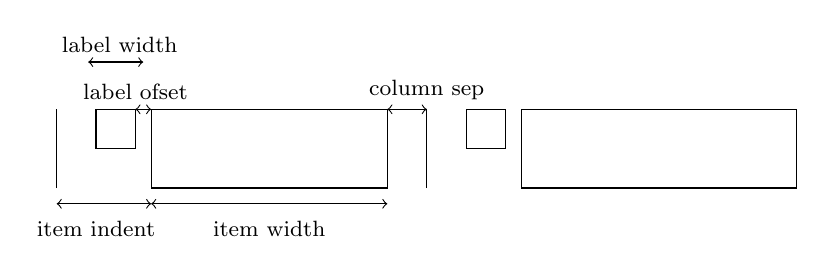
\begin{tikzpicture}
\draw(0,0)--(0,1);
\draw(-3.5,0) rectangle (-0.5,1);
\draw(0.5,0.5) rectangle (1,1);
\draw(1.2,0) rectangle (4.7,1);
\draw(-4.7,0)--(-4.7,1);
\draw(-3.7,0.5) rectangle (-4.2,1);
\draw[<->](0,1)--(-0.5,1);
\draw[<->](-3.5,1)--(-3.7,1);
\draw[<->](-4.7,-0.2)--(-3.5,-0.2);
\draw[<->](-3.5,-0.2)--(-0.5,-0.2);
\draw[<->](-3.6,1.6)--(-4.3,1.6);
\node[above] at (-3.7,1){\footnotesize label ofset};
\node[above] at (0,1){\footnotesize column sep};
\node[below] at (-4.2,-0.3){\footnotesize item indent};
\node[below] at (-2,-0.3){\footnotesize item width};
\node[above] at (-3.9,1.6){\footnotesize label width};
    \end{tikzpicture}
}
\caption{所用长度的示意图}
\end{figure}

如果:\text{indent} = \text{label}\text{width} + \text{label-offset}

即:\text{条目缩进(item indent)} = \text{标签宽度(label width)} + \text{标签偏移(label-offset)}


那么:标签(label)将与上面的文本块(textblock)对齐(如果设置了 label-align = \{left\})。请参见上述图1查看可用长度及其设置。


column-sep = {<dim>} \hfill 默认为0pt

栏间距(column sep),即两栏之间的水平间距。


label-align = left $|right|$ center \hfill 默认为 left

标签对齐(label align),设定标签(label)在标签盒子(label-box)中的对齐方式,标签盒子的宽度由 label-width 设定。

before-skip = \{<skip>\} \hfill 默认为0pt

设置列表前附加的垂直空白(before skip)。

after-skip = \{<skip>\} \hfill 默认为0pt

设置列表后附加的垂直空白(after skip)。

after-item-skip = \{<skip>\} \hfill  默认: 1ex plus 1ex minus 1ex

设置条目(items)的行(rows)之间附加的垂直空白。

resume = true$|$false \hfill 默认为 false

从以前的 tasks 环境中恢复计数(enumeration)。为了正确使用这个选项,您不应该混合使用不同的 tasks 环境,因为这些环境都会计算它们的条目。


start =\{<integer>\} \hfill 默认为 1

设置列表开始计数的起始值(starting value)。

counter = \{<counter>\} \hfill 默认为 task

设置用于计算条目(items)的计数器(counter)。

debug = true$|$false \hfill 默认为false

debug(调试)如果设置为 true,在 tasks 环境中 \verb|\|\textcolor{Tasks}{fboxsep} 将设置为 0pt,\verb|\|\textcolor{Tasks}{fbox} 将在标签盒子(label boxes)和条目盒子(item boxes)周围绘制框架(frame)。

现在,列表与上面的相同,但有三栏和一个不同的标签:

\begin{tcolorbox}[collower=black,colframe=Tasks,colback=white]
    \begin{lstlisting}
\begin{tasks}[label=(\roman * ),label-width=4ex](2)
\task \Sample
\task \sample
\task \sample
\task \Sample
\end{tasks}
\end{lstlisting}
        \tcblower
        \settasks{debug}
        \begin{tasks}[
        label=(),
        label-width=4ex
        ](2)
            \task \Sample
            \task \sample
            \task \sample
            \task \Sample
    \end{tasks}
           \end{tcolorbox}

让我们在一个问题(question)中使用它,例如,在 xsim 宏包的 exercise 环境[Nie20]中:

\begin{tcolorbox}[collower=black,colframe=Tasks,colback=white]
    \begin{lstlisting}
% 由于这些设置是局部的(local),以下设置在该示例以外将丢失;
\settasks{
label = \theexercise.\arabic * ,
item-indent = 2em ,
label-width = 2em ,
label-offset = 0pt
}
\begin{exercise}
I have these two tasks for you. Shall we begin?
\begin{tasks}(2)
\task The first task: easy!
\task The second task: even more so!
\end{tasks}
\end{exercise}
\begin{solution}[print]
Now, let's see\ldots\ ah, yes:
\begin{tasks}
\task This is the first solution. Told you it was easy.
\task This is the second solution. And of course you knew that!
\end{tasks}
\end{solution}
\end{lstlisting}
        \tcblower
% since settings are local the following ones will be lost
% outside this example;
\settasks{
   %label = \theexercise.\arabic * ,
    item-indent = 2em ,
    label-width = 2em ,
    label-offset = 0pt
    }
    I have these two tasks for you. Shall we begin?
    \begin{tasks}[style=enumerate](2)
    \task The first task: easy!
    \task The second task: even more so!
    \end{tasks}

    Now, let's see\ldots\ ah, yes:
    \begin{tasks}[style=enumerate]
    \task This is the first solution. Told you it was easy.
    \task This is the second solution. And of course you knew that!
    \end{tasks}
           \end{tcolorbox}


最后,让我们看看 debug (调试)选项的作用(您可以在第8页上看到):

\begin{tcolorbox}[collower=black,colframe=Tasks,colback=white]
    \begin{lstlisting}
\settasks{debug}
\begin{tasks}(2)
\task \Sample
\task \Sample
\end{tasks}
\end{lstlisting}
        \tcblower
        \settasks{debug}
        \begin{tasks}(2)
        \task \Sample
        \task \Sample
        \end{tasks}
           \end{tcolorbox}

\section{可用的实例}

目前,tasks 对象(tasks object)还有三个其他可用的实例:

{\bfseries itemize} 使用 \verb|\|\textcolor{Tasks}{labelitemi} 作为标签。

{\bfseries enumerate} 用 1., 2., ... 计数(enumerates)条目(items)。

\begin{tcolorbox}[collower=black,colframe=Tasks,colback=white]
    \begin{lstlisting}
\begin{tasks}[style=itemize](2)
\task that's just how\ldots
\task \ldots we expected
\end{tasks}
\begin{tasks}[style=enumerate](2)
\task that's just how\ldots
\task \ldots we expected
\end{tasks}
\end{lstlisting}
        \tcblower
        \begin{tasks}[style=itemize](2)
            \task that's just how\ldots
            \task \ldots we expected
        \end{tasks}
        \begin{tasks}[style=enumerate](2)
            \task that's just how\ldots
            \task \ldots we expected
        \end{tasks}       
\end{tcolorbox}


\section{自定义标签}

如果要更改列表中的单个标签(single label),可以使用 \verb|\|\textcolor{Tasks}{task} 命令的可选参数。

这将临时覆盖默认标签(default label)。


\begin{tcolorbox}[collower=black,colframe=Tasks,colback=white]
    \begin{lstlisting}
\begin{tasks}[style=itemize](2)
\task that's just how\ldots
\task[+] \ldots we expected
\task that's just how\ldots
\task \ldots we expected
\end{tasks}
\end{lstlisting}
        \tcblower
        \begin{tasks}[style=itemize](2)
            \task that's just how\ldots
            \task[+] \ldots we expected
            \task that's just how\ldots
            \task \ldots we expected
            \end{tasks}
           \end{tcolorbox}

您已经看到了标签选项(label option)的示例。

label = {<code>} \hfill 默认为 \verb|\|\textcolor{Tasks}{alph *} )

用于设置列表的标签(label)。其中 * 常由括号内的当前计数器名称替换。它可以包含 \verb|\|\textcolor{Tasks}{bfseries} 之类的格式化指令,但使用下面的标签格式化(label-format)选项更简洁。

label-format = {<code>}\hfill (初始为空)

这一点尤其如此,因为在您通常不希望有格式化命令(formatting instructions)的地方设置 \verb|\|\textcolor{Tasks}{the<counter>}。解决这个问题的另一种方法是使用下面的 ref 选项:

ref = {<code>}\hfill (初始为空)

该选项设置 \verb|\|\textcolor{Tasks}{the hcounteri}(\verb|\|\textcolor{Tasks}{thetask} 在默认设置里)。

\begin{tcolorbox}[collower=black,colframe=Tasks,colback=white]
    \begin{lstlisting}
\begin{tasks}[label=\arabic * .,ref=\arabic * ]
\task first item
\task second item \label{foo}
\end{tasks} See item~\ref{foo} without dot.
\end{lstlisting}
        \tcblower
        \begin{tasks}[
            %label=\arabic * .,
           % ref=\
            %arabic *
            ]
            \task first item
            \task second item \label{foo}
            \end{tasks}
            See item~\ref{foo} without dot.
           \end{tcolorbox}

定义了另外两个在某些情况下可能有用的命令:

\verb|\|\textcolor{Tasks}{tasksifmeasuringTF\{<true>\}\{<false>\}}

该命令在标签内部使用,检查标签的排版是否用于测量其宽度,或者是否为“真正的(for real)”排版。这里还有 \verb|\|\textcolor{Tasks}{tasksifmeasuringT} 变量(variants)和 \verb|\|\textcolor{Tasks}{tasksifmeasuringF} 变量。

\verb|\|\textcolor{Tasks}{tasklabel}

用于保存当前标签文本(label text)。

\section{新的tasks类(tasks-like)环境}

可以添加与 tasks 环境类似的自定义环境(custom environments)。

\verb|\|\textcolor{Tasks}{NewTasksEnvironment[<options>]\{<name>\}[<separator>](<cols>)}

使用名为 ⟨separator⟩ 的分隔符定义名为 ⟨name⟩ 的新环境。分隔符 ⟨separator⟩ 默认为\task,栏数 ⟨cols⟩ 默认为1。选项 ⟨options⟩ 在第4节中已描述。

\verb|\|\textcolor{Tasks}{RenewTasksEnvironment[<options>]\{<name>\}[<separator>](<cols>)}

用 \verb|\|\textcolor{Tasks}{NewTasksEnvironment} 修改(renew)前面定义的环境。

tasks 环境定义如下:

\begin{tcolorbox}[collower=black,colframe=Tasks,colback=white]
    \begin{lstlisting}
    \NewTasksEnvironment{tasks}
    \end{lstlisting}
\end{tcolorbox}

分隔符(separator)不必是控制序列(control sequence):

\begin{tcolorbox}[collower=black,colframe=Tasks,colback=white]
    \begin{lstlisting}
% preamble:
% \usepackage{fontawesome}
\NewTasksEnvironment[label=\faThumbsOUp,label-width=15pt]{done}[ * ]
\begin{done}
* First task
* Second task
\end{done}
\end{lstlisting}
        \tcblower
        %\NewTasks[style=\footnotesize\leftthumbsup,label-width=1.3em]{done}[ * ]
\begin{tasks}(2)
\task[$\clubsuit$] First task
\task[$\spadesuit $] Second task
\task[$\surd $] First task
\task[$\heartsuit $] Second task
\end{tasks}
\end{tcolorbox}

虽然这看起来很方便,甚至很好,但我强烈建议不要使用与命令序列(command sequence)不同的东西。记住,每当出现分隔符(separator)时,条目(items)都会被拆分。因此,为了在一个条目(items)中使用分隔符(separator)(例如,这里是一个带星号的命令变体),它必须隐藏在中括号中。这可以避免你使用一个还未定义的命令序列。

还请记住,分隔符(separator)仍然有一个可选的星号参数(optional star argument)(参见4)、一个可选的感叹号参数(optional bang argument)和标准可选参数(standard optional argument)。使用*将阻止可选的星号参数。

\begin{tcolorbox}[collower=black,colframe=Tasks,colback=white]
    \begin{lstlisting}
% preamble:
% \usepackage{fontawesome}
\NewTasksEnvironment[label=\faThumbsOUp,label-width=15pt]{done}[ * ]
\begin{done}(3)
* First task
* Second task
* ! Third task spanning the full width available
* Fourth task
\end{done}
\end{lstlisting}
        \tcblower
        %\NewTasksEnvironment[label=\faThumbsOUp,label-width=15pt]{done}[ * ]
\begin{tasks}(2)
\task[$\nabla $] First task
\task[>>>>] Second task
\end{tasks}
           \end{tcolorbox}


\section{样式化 tasks}

TASK 使用 xtemplate 宏包为列表声明其它实例(additional instances)。

\subsection{tasks 对象}

由 tasks 定义的对象(object)是“tasks”对象。这一次,定义的一个模板(同样是“默认”)有四个实例可用。

\subsubsection{可用的选项}

本节仅列出定义“defaul”模板的实例时可用的选项。下面的内容给出了一些例子。

\begin{tcolorbox}[collower=black,colframe=Tasks,colback=white]
    \begin{lstlisting}
\DeclareTemplateInterface{tasks}{default}{3}{
% option : type = default
label : tokenlist = \alph * ) ,
indent : length = 2.5em ,
label-format : tokenlist ,
label-width : length = 1em ,
label-offset : length = .3333em ,
after-item-skip : skip = 1ex plus 1ex minus 1ex
}
\end{lstlisting}
    \end{tcolorbox}

\subsubsection{预定义的实例}

这一次相当简洁:

    \begin{tcolorbox}[collower=black,colframe=Tasks,colback=white]
        \begin{lstlisting}
% alphabetize: a) b) c)
\DeclareInstance{tasks}{alphabetize}{default}{}
% itemize
\DeclareInstance {tasks} {itemize} {default}{
label-width = 1.125em ,
label = \labelitemi}  % enumerate:
\DeclareInstance {tasks} {enumerate} {default}
{label = \arabic * . }
    \end{lstlisting}
        \end{tcolorbox}

\begin{thebibliography}{9}

\bibitem{1} Javier Bezos. enumitem. Version 3.9. June 20, 2019. url: https://ctan.org/pkg/enumitem.

\bibitem{2} The \LaTeX{}3 Project Team. l3kernel. Sept. 19, 2019.
url: https://www.ctan.org/pkg/ l3kernel/.

\bibitem{3} Clemens Niederberger. exsheets. Version 0.21k. Sept. 30, 2019.
url: https://ctan. org/pkg/exsheets.

\bibitem{4} Clemens Niederberger. xsim. Version 0.19a. Mar. 19, 2020.
url: https://ctan.org/pkg/xsim.

\bibitem{5} Will Robertson. environ. Version 0.3. May 4, 2014.
url: https://ctan.org/pkg/environ .

\end{thebibliography}
\end{document} 
